\chapter{Mở đầu}
% \addcontentsline{toc}{chapter}{Mở đầu}
\setcounter{page}{1}
\pagenumbering{arabic}
\section{Giới thiệu}

\subsection{Vi khuẩn, vi-rút, thực khuẩn và vùng protein bảo tồn}

Vi khuẩn là sinh vật đơn bào có kích thước nhỏ (0,2 - 5 µm), có cấu tạo đơn giản bao gồm tế bào chất, màng tế bào và vách tế bào. Vi khuẩn sinh sản chủ yếu bằng phương pháp phân đôi. Ngược lại, vi-rút không phải là sinh vật sống hoàn chỉnh do không có cấu trúc tế bào, mà chỉ bao gồm vật liệu di truyền (ADN hoặc ARN) được bao bọc bởi lớp vỏ protein. Vi-rút chỉ có thể sao chép khi xâm nhập vào tế bào vật chủ và khai thác bộ máy sinh học của tế bào đó.

Trong nhóm vi-rút, \textbf{thực khuẩn} là loại xâm nhiễm vào vi khuẩn. Mỗi loại vi khuẩn thường bị nhiễm bởi một hoặc một vài loại thực khuẩn đặc trưng. Thực khuẩn đóng vai trò quan trọng trong điều hòa quần thể vi khuẩn tự nhiên và đang được nghiên cứu ứng dụng trong y học. Dựa trên chu kì sống bên trong vi khuẩn, thực khuẩn được chia thành hai nhóm chính: \textbf{Thực khuẩn thể độc lực} và \textbf{thực khuẩn thể ôn hoà}. Với thực khuẩn thể độc lực, sau khi xâm nhập vào tế bào vi khuẩn, thực khuẩn chiếm quyền kiểm soát, nhân bản, và phá hủy tế bào để giải phóng các bản sao mới, quá trình này được gọi là \textbf{chu kỳ tan}. Với thực khuẩn thể ôn hoà, chúng tích hợp vật liệu di truyền của mình vào hệ gen của vi khuẩn, nhân bản cùng vật chủ mà không phá hủy tế bào, quá trình này gọi là \textbf{chu kỳ tiền tan} và có thể chuyển sang chu kỳ tan khi gặp điều kiện kích hoạt.

Vùng protein bảo tồn trong bộ gen thực khuẩn là các vùng chức năng trong chuỗi axit amin của protein, được duy trì qua quá trình tiến hóa và thường xuất hiện ở nhiều loài thực khuẩn khác nhau. Những protein này thường liên quan đến các chức năng thiết yếu như lắp ráp cấu trúc vi-rút, xâm nhập tế bào chủ, sao chép dữ liệu di truyền và ly giải tế bào vi khuẩn.


\subsection{Động lực thúc đẩy}

Việc phân loại thực khuẩn là có độc lực hay ôn hòa mang đến những lợi ích to lớn cho việc nghiên cứu hệ vi sinh vật và ứng dụng của chúng. Đầu tiên, phân loại thực khuẩn là chìa khóa để khám phá mối quan hệ phức tạp giữa thực khuẩn và vật chủ, từ đó làm sáng tỏ vai trò của thực khuẩn trong cộng đồng vi sinh vật. Tiếp theo, việc nhận diện chính xác thực khuẩn có độc lực là bước đệm quan trọng cho việc phát triển các liệu pháp điều trị bằng thực khuẩn, nhằm tiêu diệt các vi khuẩn gây bệnh, mở ra hướng đi mới cho việc điều trị.

Để phân loại một thực khuẩn mới có thuộc thể độc lực hay ôn hòa, phương pháp truyền thống là nuôi cấy trong phòng thí nghiệm và theo dõi. Các kỹ thuật nuôi cấy này không chỉ tốn thời gian và chi phí mà còn không có khả năng áp dụng được đối với các trình tự thực khuẩn mới được tổng hợp từ môi trường. Do đó, một phương pháp phân loại thực khuẩn dựa trên tính toán thông qua dữ liệu trình tự gen của thực khuẩn là cần thiết.

Với mục tiêu cải tiến phương pháp cũ hay phát triển phương pháp mới, báo cáo này cung cấp một góc nhìn tổng quan về các phương pháp tiêu biểu đã được công bố, giúp tiếp cận bài toán phân loại thực khuẩn dựa trên tính toán một cách khái quát và nhanh chóng nhất.

\section{Phát biểu bài toán}

Trong bối cảnh số lượng lớn thực khuẩn được phát hiện thông qua các công nghệ giải trình tự thế hệ mới, việc phân loại thực khuẩn bằng các phương pháp truyền thống là rất tốn kém, về cả nguồn lực và tài chính. Cùng với sự phát triển của công nghệ tính toán, các phương pháp học máy và học sâu được sử dụng để thực hiện phân loại thực khuẩn.

\subsection{Định nghĩa bài toán}
\begin{figure}[H]
    \centering
    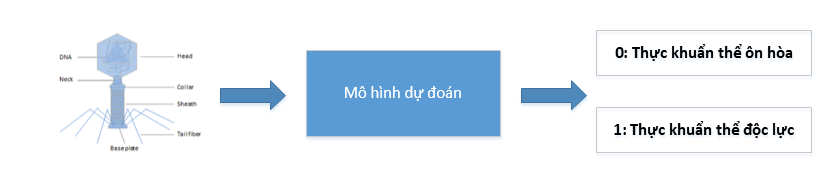
\includegraphics[width=1\linewidth]{figures/problem.png}
    \caption{Sơ đồ mô tả bài toán phân loại thực khuẩn dựa trên tính toán}
    \label{fig:problem}
\end{figure}

Hình \ref{fig:problem} mô tả bài toán phân loại thực khuẩn dựa trên phương pháp tính toán, trong đó:
\begin{itemize}
    \item \textbf{Dữ liệu đầu vào}: Chuỗi DNA đầy đủ hoặc tập hợp các đoạn DNA ngắn được lấy từ bộ gen của thực khuẩn.
    \item \textbf{Mô hình dự đoán}: Thuật toán học máy, học sâu được huấn luyện.
    \item \textbf{Dữ liệu đầu ra}: Dự đoán thực khuẩn là thể có độc lực hay thể ôn hòa.
\end{itemize}

\subsection{Đặc điểm của bài toán}

\begin{itemize}
    \item Xét ở khía cạnh học máy, bài toán phân loại thực khuẩn là bài toán phân loại nhị phân.
    \item Dữ liệu đầu vào có độ dài và chất lượng không đồng đều, bao gồm cả các trình tự ngắn hoặc có chứa nhiễu sinh học.
    \item Các mô hình cần đảm bảo tính chính xác cao, khả năng khái quát tốt với dữ liệu chưa thấy trong quá trình huấn luyện.
    \item Phải xử lý được dữ liệu có nguồn gốc từ các họ thực khuẩn khác nhau và có tính đa dạng về mặt di truyền học.
\end{itemize}

\subsection{Thách thức trong quá trình thực hiện}
Với cách tiếp cận dựa trên tính toán, việc phân loại thực khuẩn hiện tại đang gặp phải 4 khó khăn chính:
\begin{enumerate}
    \item \textbf{Thiếu dữ liệu huấn luyện chất lượng cao}: Mặc dù số lượng thực khuẩn trong tự nhiên được ước tính lên đến khoảng $10^{31}$ \cite{doi:10.1128/jb.00052-20}, nhưng hiện nay chỉ có một lượng rất nhỏ bộ gen thực khuẩn đã được giải trình tự hoàn chỉnh và đưa vào cơ sở dữ liệu. Phần lớn các thực khuẩn này vẫn chưa được xác định đặc điểm sinh học cụ thể, bao gồm cả thông tin về vòng đời (chu kỳ sinh tan hay tiềm tan). Điều này dẫn đến sự thiếu hụt dữ liệu được gán nhãn rõ ràng và chính xác, gây khó khăn cho quá trình huấn luyện các mô hình học máy trong bài toán phân loại vòng đời thực khuẩn.
    \item \textbf{Không tồn tại chỉ dấu sinh học phổ quát}: Không giống như vi khuẩn có gen 16S rRNA được bảo tồn cao, đóng vai trò như một chỉ dấu phân tử phổ quát trong phân loại và phân tích phát sinh loài, thực khuẩn không sở hữu bất kỳ gen nào có mặt đồng nhất và bảo tồn trên toàn bộ các nhóm thực khuẩn \cite{PMID:31061483}. Do đó, việc phân loại thực khuẩn thường dựa trên nội dung bộ gen hoặc các gen đặc trưng cho từng nhóm nhỏ.
    \item \textbf{Tính tương đồng di truyền với vật chủ}: Nhiều đoạn gen của phage có thể có trình tự tương tự hoặc thậm chí đồng nhất với gen vi khuẩn, do quá trình tiến hóa đồng hành hoặc sự trao đổi gen thông qua cơ chế di truyền ngang.
    \item \textbf{Xử lý dữ liệu không đầy đủ}: Trong những nghiên cứu gần đây, dữ liệu được thu thập thông qua metagenomics – phương pháp giải trình tự toàn bộ DNA có trong mẫu môi trường (như đất, nước, ruột sinh vật) mà không cần phải nuôi cấy vi sinh vật trong phòng thí nghiệm. Tuy nhiên, một đặc điểm hạn chế của phương pháp này là chỉ thu được các đoạn DNA ngắn, rời rạc và không hoàn chỉnh, thay vì toàn bộ bộ gen đầy đủ của một loại thực khuẩn. Điều này gây khó khăn vì các đoạn trình tự thu được có thể không chứa đủ thông tin đặc trưng, dễ bị nhiễu hoặc nhầm lẫn với vật liệu di truyền từ các sinh vật khác trong mẫu. Do đó, việc xử lý dữ liệu từ metagenomics đòi hỏi các phương pháp phân tích chuyên biệt để bù đắp cho tính không đầy đủ và phân mảnh của dữ liệu..
\end{enumerate}

Với các đặc điểm nêu trên, bài toán phân loại thực khuẩn đòi hỏi sự kết hợp giữa kiến thức sinh học phân tử và các kỹ thuật trong lĩnh vực học máy và học sâu. Đây chính là trọng tâm của các phương pháp được khảo sát trong báo cáo này.

\section{Nguồn dữ liệu và định dạng dữ liệu}

\subsection{Nguồn dữ liệu}

Các phương pháp phân loại được đề cập đến trong báo cáo này lấy dữ liệu từ các nguồn sau:

\begin{itemize}
    \item \textbf{NCBI (National Center for Biotechnology Information - \url{https://www.ncbi.nlm.nih.gov/})}: Là một trong những kho dữ liệu sinh học lớn và toàn diện nhất, chứa thông tin về trình tự DNA, protein, gen, và các chú thích liên quan. NCBI cung cấp cả dữ liệu thô và đã được gán nhãn, là nguồn phổ biến cho việc huấn luyện và đánh giá mô hình phân loại.
    
    \item \textbf{PhageScope - \url{https://phagescope.deepomics.org/database}}: Là cơ sở dữ liệu chuyên biệt dành cho thực khuẩn, hỗ trợ phân tích chức năng, xác định vòng đời và các đặc điểm phân tử. PhageScope tích hợp các công cụ tính toán, hỗ trợ xử lý và khám phá dữ liệu thực khuẩn ở mức độ chi tiết.
    
    \item \textbf{PhageDB - \url{https://phagesdb.org}}: Là kho dữ liệu tập trung vào thu thập và lưu trữ thông tin thực nghiệm về các chủng thực khuẩn đã được phát hiện. PhageDB thường được sử dụng để đánh giá mô hình phân loại trên các bộ dữ liệu thực tế.
\end{itemize}

\subsection{Định dạng dữ liệu}

Khi xử lý dữ liệu thực khuẩn, hai định dạng tập tin phổ biến là \texttt{FASTA} và \texttt{GenBank}. Mỗi định dạng cung cấp một cách biểu diễn riêng cho trình tự nucleotide và thông tin liên quan.

\subsubsection{Định dạng FASTA}

Định dạng \texttt{FASTA} là định dạng văn bản đơn giản dùng để lưu trữ trình tự nucleotide hoặc amino acid. Tệp tin định dạng FASTA có phần mở rộng là *.fasta. Cấu trúc của tập tin FASTA bao gồm hai phần:

\begin{itemize}
    \item \textbf{Dòng tiêu đề} (header): Bắt đầu bằng ký tự \texttt{>}, tiếp theo là thông tin mô tả, thường bao gồm ID chuỗi, tên sinh vật, tên gen hoặc nguồn gốc.
    \item \textbf{Trình tự} (sequence): Nằm ở các dòng tiếp theo, chứa các ký tự đại diện cho nucleotide (\texttt{A}, \texttt{T}, \texttt{G}, \texttt{C}) hoặc acid amin.
\end{itemize}

\noindent Ví dụ: file $NC\_000866\_Lytic.fasta$ có nội dung như sau:
\begin{verbatim}
>NC_000866.4 Enterobacteria phage T4, complete genome
AATTTTCCTTATTAGGCCGCAAGGGCCTTCATAGTTTTAGCGATTTGGGAAACTTCATCA
TCACTTAAAGAGTTGCGATAACCGATGAAGTCGGAAACAATACGGAATTTCTTGGTAAAC
TCAGCAACCATTTTATCACTGTTTTTTGAAGCATTATTTGATAATACATCAAAAAGATTA
GTTACTGTCCAAATGTCATGACCGATGGTATCTTTTCCACCATTAAAATATACACCCTGT
.....
\end{verbatim}

\subsubsection{Định dạng GenBank}

Định dạng \texttt{GenBank} là định dạng tiêu chuẩn của NCBI, chứa thông tin chi tiết hơn so với FASTA. Tệp tin định dạng FASTA có phần mở rộng là *.gb.  Một tệp tin GenBank bao gồm ba phần chính:

\begin{itemize}
    \item \textbf{Phần tiêu đề} (Header): Mô tả chung về bộ gen, bao gồm số hiệu truy cập, nguồn sinh vật, độ dài chuỗi và các đặc điểm chung.
    \item \textbf{Phần đặc trưng} (Features): Liệt kê các đặc trưng sinh học của chuỗi, bao gồm vị trí gen, loại protein mã hóa, chú thích chức năng.
    \item \textbf{Phần trình tự} (Sequence): Trình bày toàn bộ chuỗi nucleotide của bộ gen.
\end{itemize}

Ví dụ dưới đây là một phần của file $AF503408\_Lysogneic.gb$
\begin{verbatim}
LOCUS       AF503408    101660 bp    DNA     linear   PHG 28-APR-2006
DEFINITION  Enterobacteria phage P7, complete genome.
ACCESSION   AF503408
.....
FEATURES             Location/Qualifiers
     source          1..101660
                     /organism="Enterobacteria phage P7"
                     /mol_type="genomic DNA"
                     /db_xref="taxon:10682"
....
ORIGIN      
  1 acattatacg aagttatatt aagggttatt gaacatgatc aatttacctg taaatccata
 61 cagttcaata ccttatcagg tcaaatagtg atcacttgat catttgatca agtttgcgct
121 acgtaaaatc tgtgaaaagt tggcagtgtt agtgctccag atttcgcgta gcgcacttag
181 caccaccaat caatcagagg tgaaaaatgg gatattcagc tgctaaagtg tccactcatc
241 ttgagcttga gaaaaaccgt ggttactggc gggcaaaagg gtttgatcgt gatagttgcc
301 aactgtcatt atcgcgcggt gaagagaaaa tagtacgcac gcgcggtcgc tggcgtttct
\end{verbatim}


Định dạng GenBank hỗ trợ các phần mềm sinh học phân tử và hệ thống phân tích chú thích gen trong quá trình tiền xử lý dữ liệu.

\cleardoublepage